\documentclass[10pt,twocolumn]{article}

\usepackage[utf8]{inputenc}
\usepackage[T1]{fontenc}
\usepackage[provide=*,italian]{babel}
\usepackage{lmodern}
\usepackage[protrusion=true,expansion=false]{microtype}
\usepackage[a4paper, top=1.9cm, bottom=1.9cm, left=1.65cm, right=1.65cm, columnsep=0.65cm]{geometry}
\usepackage{amsmath, amssymb, amsfonts, amsthm}
\usepackage{graphicx}
\usepackage{booktabs}
\usepackage{xcolor}
\usepackage{hyperref}
\usepackage{enumitem}

\definecolor{linkblue}{RGB}{20, 70, 140}
\hypersetup{
    colorlinks=true,
    linkcolor=linkblue,
    citecolor=linkblue,
    urlcolor=linkblue,
    pdftitle={HySA: Architettura Semantica Ibrida},
    pdfauthor={Francesco Mariani}
}

\newtheorem{proposition}{Proposizione}
\theoremstyle{definition}
\newtheorem{definition}{Definizione}

\title{\vspace{-1.0cm}\textbf{\Large HySA (Hybrid Semantic Architecture): Preservare l'Astrazione Polisemantica tramite Tensori d'Inferenza a Contrasto, Indicizzazione Monosemantica e Temperatura Topologica \texorpdfstring{($T_t$)}{(Tt)}}}

\author{
    \textbf{Francesco Mariani} \\
    \textit{Independent Systems Architect} \\
    Umbria, Italia \\
    \texttt{fratorials@gmail.com} \\
    {\footnotesize DOI: \href{https://doi.org/10.5281/zenodo.23456159}{\texttt{10.5281/zenodo.23456159}}}
}

\date{Ottobre 2026}

\begin{document}

\twocolumn[
  \begin{@twocolumnfalse}
    \maketitle
    \begin{center}
        \vspace{-0.35cm}
        \textit{``L'industria dell'IA vede il polisemantismo come una condanna... ma forse è la benedizione che ha reso tutto possibile.''}
        \vspace{0.25cm}
    \end{center}
    \begin{abstract}
      \noindent La ricerca contemporanea sull'\textit{Interpretabilità Meccanicistica} tratta prevalentemente la polisemia neuronale come un artefatto indesiderato della compressione dimensionale (\textit{Ipotesi della Superposizione}), concentrandosi sulla scomposizione degli spazi latenti in vasti dizionari sparsi di feature puramente monosemantiche. In questo lavoro proponiamo un cambio di paradigma: \textbf{la polisemia non è un difetto da sradicare, ma il prerequisito geometrico per l'intelligenza e il ragionamento analogico.} Un neurone puramente monosemantico è intrinsecamente ``stupido'' ($\emptyset$ intelligenza): privo di connessioni associative trasversali, funziona come una cella di memoria rigorosa ma sterile. Per disaccoppiare il comportamento associativo fluido dalla verifica fattuale deterministica senza ricorrere ad architetture in serie (che introducono colli di bottiglia non astrattivi) o reti in parallelo (computazionalmente inefficienti), introduciamo \textbf{HySA (\textit{Hybrid Semantic Architecture})}, un paradigma unificato delimitato dalla semanticità neuronale. HySA introduce quattro contributi fondamentali: (1) la \textbf{Superposizione d'Inferenza a Contrasto} ($I_n$), che estrae il cubo multi-concettuale delle unità polisemantiche tramite aspettative d'inferenza ponderate su dataset a contrasto; (2) l'\textbf{Indicizzazione Monosemantica}, che accoppia una rete polisemantica ($N_p$, intelligenza) con un registro indicizzato di centroidi monosemantici ($N_m / N_k$, memoria) interrogato tramite API interne deterministiche; (3) l'\textbf{Ipersfera Semantica}, governata da una doppia temperatura ($T_p, T_m$) e dalla \textbf{Temperatura Topologica} ($T_t$); e (4) il \textbf{Gradiente di Compressione} ($\Delta q$) tra $N_p$ e $N_m$, regolato dal Grado di Determinismo $\beta = T/q$ attorno a un \textbf{Punto Critico} stazionario ($P_c$).
      \vspace{0.35cm}
    \end{abstract}
  \end{@twocolumnfalse}
]

\section{Introduzione: Intelligenza vs. Memoria}
Nelle reti neurali profonde, le singole unità esibiscono costantemente \textit{selettività mista}~\cite{rigotti2013importance, elhage2022toy}. Gli approcci prevalenti basati su \textit{Sparse Autoencoders} (SAE)~\cite{bricken2023monosemanticity, templeton2024scaling} cercano di separare queste rappresentazioni in dimensioni ortogonali e monosemantiche. Tuttavia, questa ricerca della monosemia pura trascura una divisione epistemologica fondamentale tra \textbf{Intelligenza} e \textbf{Memoria}:
\begin{itemize}[leftmargin=*, itemsep=1.5pt, topsep=2pt]
    \item \textbf{I Neuroni Polisemantici} ($N_p$) \textbf{Generano l'Intelligenza:} Un'unità che si co-attiva attraverso concetti quali \texttt{IP}, \texttt{DNS}, \texttt{Pagine Bianche} e \texttt{Numero di Telefono} non sta subendo un'interferenza rumorosa. Sta comprimendo più concetti in un significato unificato di ordine superiore: lo schema relazionale della \textit{risoluzione identità-indirizzo}. \textbf{I collegamenti associativi sono ciò che rende intelligente un sistema.}
    \item \textbf{I Neuroni Monosemantici} ($N_m$) \textbf{Forniscono la Memoria:} Le unità che codificano letterali atomici rigidi---come l'indirizzo IP \texttt{8.8.8.8}, l'intero \texttt{24} o il nome proprio \texttt{JOHN}---possiedono zero connessioni associative ($\emptyset$ intelligenza). Come le voci di un dizionario statico, un'unità monosemantica è cognitivamente ``stupida'', ma è \textbf{strettamente rigorosa}---rendendola essenziale per prevenire le allucinazioni.
\end{itemize}

I moderni LLM allucinano perché aggrovigliano entrambi i regimi all'interno delle stesse matrici di pesi omogenee~\cite{geva2021transformer}, permettendo ai gradienti associativi di interpolare attraverso fatti immutabili.

\begin{figure*}[t]
    \centering
    \IfFileExists{fig1_imprinted_tensors.pdf}{
        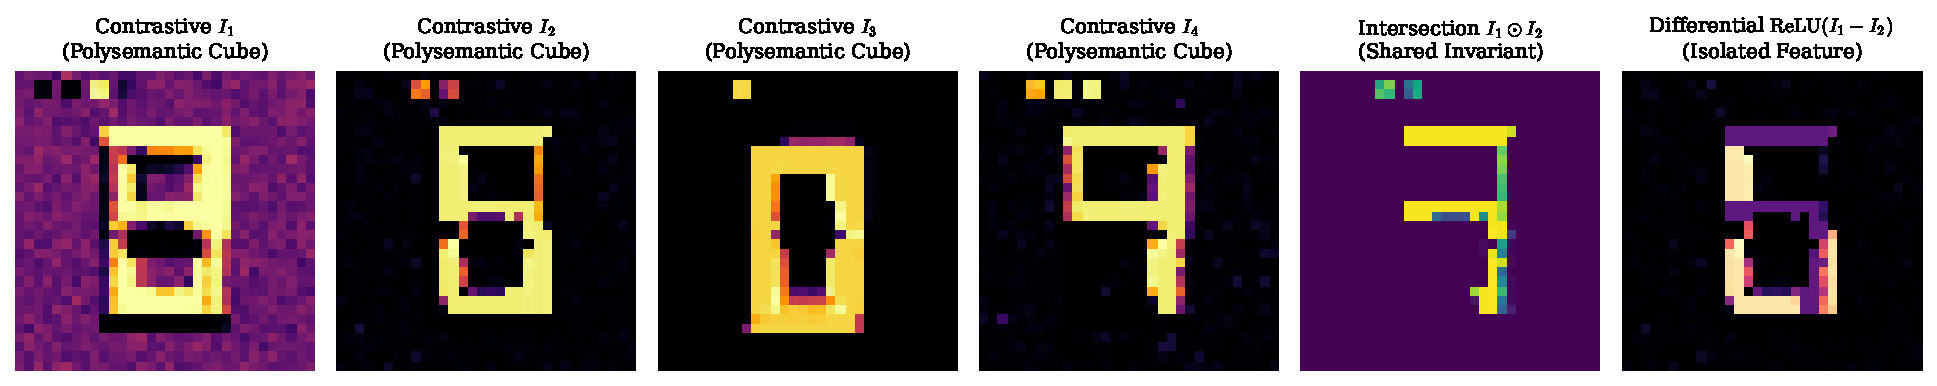
\includegraphics[width=0.98\textwidth]{fig1_imprinted_tensors.pdf}
    }{
        \fbox{\parbox{0.95\textwidth}{\centering \vspace{0.8cm} \textbf{[Figura 1]} \vspace{0.8cm}}}
    }
    \vspace{-0.15cm}
    \caption{\textbf{Tensori di Superposizione a Contrasto ($I_n$) e Query Semantiche Algebriche sul Benchmark $32 \times 32$.} Le colonne 1--4 mostrano le rappresentazioni polisemantiche apprese da un collo di bottiglia a 4 neuroni. La colonna 5 isola l'invariante condivisa ($I_1 \odot I_2$). La colonna 6 estrae la divergenza differenziale della feature ($\mathrm{ReLU}(I_1 - I_2)$).}
    \label{fig:imprinted_tensors}
\end{figure*}

\section{Chiarimento sulla Terminologia di Sistema}
Ogni unità indicizzata $N_k$ possiede un centroide monosemantico $\mu_k$ strutturalmente analogo a un \textbf{``Inode''} di un sistema operativo, il che motiva il nostro utilizzo del termine \textbf{``Filesystem''}. Per prevenire ambiguità interdisciplinari, la Tabella~\ref{tab:terminology} mappa queste euristiche di sistema nei rispettivi costrutti matematici formali nello spazio latente $\mathcal{S} \subset \mathbb{R}^D$.

\begin{table}[h]
\centering
\caption{Mappatura delle Euristiche di Sistema nei Costrutti Formali.}
\label{tab:terminology}
\vspace{0.15cm}
\scriptsize
\begin{tabular}{@{}p{1.9cm}p{2.3cm}p{3.0cm}@{}}
\toprule
\textbf{Termine OS} & \textbf{Costrutto Formale} & \textbf{Ruolo Architetturale} \\ \midrule
\textbf{``Inode''} ($N_k$) & Centroide $\mu_k \in \mathbb{R}^D$ & Puntatore ortogonale a un letterale atomico immutabile (es. \texttt{8.8.8.8}). \\[3pt]
\textbf{``Filesystem''} & Varietà Indicizzata $\mathcal{F}_{\mathrm{mono}} = \{\mu_1, \dots, \mu_M\}$ & Storage a dizionario ($\emptyset$ intelligenza, $100\%$ rigore) per la verifica. \\[3pt]
\textbf{``Query / API''} & Operatore Metrico $Q(q, \mathcal{F}_{\mathrm{mono}}, T_t)$ & Controllo di confine deterministico che conferma gli stati polisemantici. \\ \bottomrule
\end{tabular}
\end{table}

\section{Tensori di Superposizione a Contrasto \texorpdfstring{($I_n$)}{(In)}}
Un neurone polisemantico agisce come un cubo di superposizione ad alta dimensionalità che comprime molteplici concetti in significati unificati. Poiché un neurone isolato è uno scalare muto, la sua geometria interna viene estratta come la \textbf{media ponderata di tutti i risultati delle inferenze attraverso un dataset a contrasto} ($\mathcal{X}^+$ contenente invarianti strutturali condivise vs. baseline $\mathcal{X}^-$):
\begin{equation}
\begin{aligned}
    I_n = \frac{1}{\sum_{k} z_{k,n} + \eta} \bigg[ & \sum_{X_k \in \mathcal{X}^+} z_{k,n} \cdot \Phi_{\mathrm{net}}(X_k \mid n) \\
    & - \gamma \sum_{X_j \in \mathcal{X}^-} z_{j,n} \cdot \Phi_{\mathrm{net}}(X_j \mid n) \bigg]
\end{aligned}
\label{eq:imprinted_tensor}
\end{equation}
dove $z_{k,n}$ è l'attivazione dell'unità $n$ e $\Phi_{\mathrm{net}}(\cdot \mid n)$ è l'inferenza dell'intera rete condizionata su $n$. Le invarianti condivise sono interrogate tramite $I_A \odot I_B$ e le divergenze tramite $\mathrm{ReLU}(I_A - I_B)$ (Figura~\ref{fig:imprinted_tensors}).

\section{Il Paradigma Ibrido Unificato (HySA)}
Come devono interagire l'intelligenza polisemantica ($N_p$) e la memoria monosemantica ($N_m$)?
\begin{itemize}[leftmargin=*, itemsep=1.5pt, topsep=2pt]
    \item \textbf{Né in Serie:} Posizionare uno strato monosemantico rigido a valle di $N_p$ crea un \textit{collo di bottiglia non astrattivo} che distrugge le relazioni contestuali.
    \item \textbf{Né in Parallelo:} Eseguire reti duplicate simultaneamente è \textit{estremamente inefficiente} dal punto di vista computazionale.
\end{itemize}
In \textbf{HySA}, il modello è un \textbf{tutt'uno unificato}, delimitato internamente dalla logica e dalla specifica ``semanticità'' (dimensionalità e cardinalità $M$) dei singoli neuroni dentro i layer. Il ragionamento fluido si propaga attraverso $N_p$; quando è richiesta una conferma fattuale, la traiettoria esegue una concisa \textbf{Query/API} interna verso i centroidi monosemantici indicizzati $\mathcal{F}_{\mathrm{mono}}$, conferendo consistenza deterministica.

\begin{figure*}[t]
    \centering
    \IfFileExists{fig2_phase_transition.pdf}{
        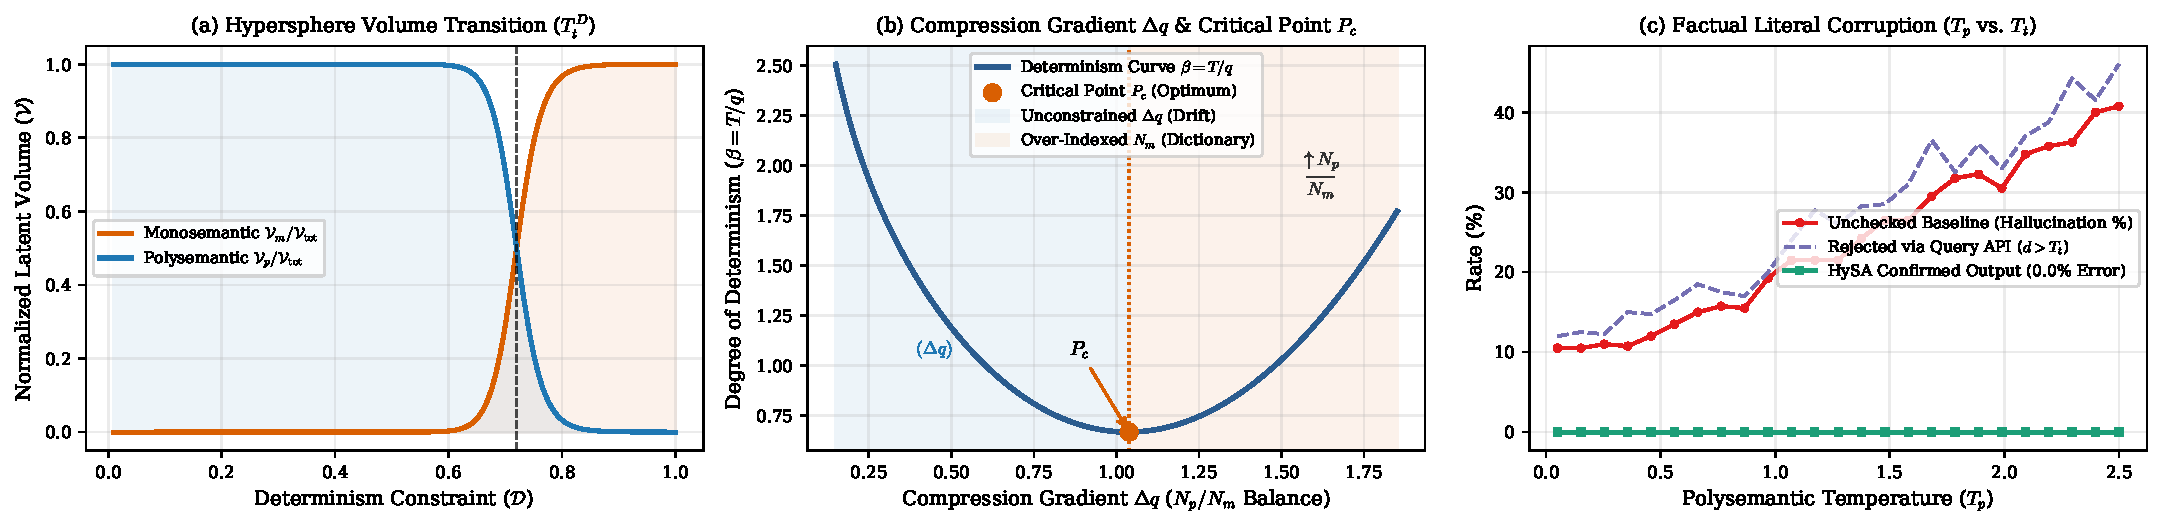
\includegraphics[width=0.98\textwidth]{fig2_phase_transition.pdf}
    }{
        \fbox{\parbox{0.95\textwidth}{\centering \vspace{0.8cm} \textbf{[Figura 2]} \vspace{0.8cm}}}
    }
    \vspace{-0.15cm}
    \caption{\textbf{Transizione di Fase del Volume ad Alta Dimensionalità, Punto Critico ($P_c$) e Verifica Fattuale in HySA.} \textbf{(a)} Transizione a gradino tra il Volume Polisemantico Libero $\mathcal{V}_p$ e il Volume di Vincolo Monosemantico $\mathcal{V}_m$. \textbf{(b)} Curva di potenziale del gradiente di compressione $\Delta q$ che mostra il Punto Critico stazionario $P_c$ rispetto a $\beta = T/q$. \textbf{(c)} Il decoding non controllato subisce una corruzione fattuale crescente, mentre HySA mantiene lo $0.0\%$ di corruzione tramite conferma API monosemantica entro $T_t$.}
    \label{fig:phase_transition}
\end{figure*}

\section{L'Ipersfera Semantica e la Doppia Temperatura \texorpdfstring{($T_p, T_m, T_t$)}{(Tp, Tm, Tt)}}
Anziché applicare la temperatura come rumore post-hoc sulla \textit{Softmax}, HySA definisce geometricamente la temperatura come \textbf{l'intorno multidimensionale del neurone}: un'\textbf{Ipersfera Semantica} nello spazio latente.

Quando una traiettoria latente viene \textit{interrogata} all'interno di questa ipersfera (dove token o concetti correlati come \texttt{CAT}, \texttt{GATTO}, \texttt{KG} o \texttt{MACCHINA} giacciono lungo vettori radiali $A, B, C, D$), la dinamica del sistema è governata da due temperature di regime---la \textbf{Temperatura Polisemantica} ($T_p$) e la \textbf{Temperatura Monosemantica} ($T_m$)---delimitate dalla \textbf{Temperatura Topologica} ($T_t$):
\begin{equation}
    B(\mu_k, T_t) = \left\{ x \in \mathcal{S} \;\middle|\; \| x - \mu_k \|_2 \le T_t(T_p, T_m) \right\}
\end{equation}
Se un punto interrogato $q$ cade entro il raggio $T_t$ del centroide $\mu_k$, l'API conferma il passaggio logico e vincola il letterale esatto da $\mu_k$. Se $\|q - \mu_k\|_2 > T_t$, HySA solleva un \textit{Semantic Fault} deterministico, bloccando l'allucinazione (Figura~\ref{fig:phase_transition}).

\section{Gradiente di Compressione \texorpdfstring{($\Delta q$)}{(Delta q)}, Determinismo \texorpdfstring{($\beta$)}{(beta)} e Punto Critico \texorpdfstring{($P_c$)}{(Pc)}}
Il rapporto strutturale tra neuroni polisemantici ($N_p$) e centroidi monosemantici ($N_m$) definisce il \textbf{Gradiente di Compressione} ($\Delta q$) attraverso i layer. Sia $q = f(N_p, N_m, M)$ la quantità neuronale effettiva. Definiamo il \textbf{Grado di Determinismo} ($\beta$) come:
\begin{equation}
    \beta = \frac{T}{q}
\end{equation}
Mappare $\beta$ rispetto al gradiente di compressione $\Delta q$ genera un panorama di potenziale convesso con un minimo stazionario nel \textbf{Punto Critico} ($P_c$, Figura~\ref{fig:phase_transition}b):
\begin{enumerate}[leftmargin=*, itemsep=1.5pt, topsep=2pt]
    \item \textbf{A sinistra di $P_c$ ($\Delta q$ Sotto-Vincolato):} La dominanza di $N_p$ senza sufficiente indicizzazione $N_m$ porta a una deriva associativa non ancorata.
    \item \textbf{A destra di $P_c$ (Saturazione Sovra-Indicizzata):} La dominanza di $N_m$ recide i legami associativi; $\mathcal{V}_m \propto M \cdot (T_t)^D$ satura lo spazio, congelando il modello in un dizionario statico.
    \item \textbf{Nel Punto Critico ($P_c$):} Equilibrio ottimale tra $N_p$ e $N_m$, che massimizza l'astrazione polisemantica garantendo al contempo la verifica deterministica.
\end{enumerate}

\section{Validazione Sperimentale}
Validiamo HySA attraverso due benchmark complementari:
\begin{enumerate}[leftmargin=*, itemsep=1.5pt, topsep=2pt]
    \item \textbf{Benchmark a Contrasto $32 \times 32$:} Un collo di bottiglia a 4 neuroni addestrato su matrici binarie a doppia natura (anelli numerici condivisi + checksum letterali rigidi $2\times2$ in alto a sinistra). Come mostrato in Figura~\ref{fig:imprinted_tensors} e Figura~\ref{fig:phase_transition}c, le query algebriche ($I_1 \odot I_2$ e $\mathrm{ReLU}(I_1 - I_2)$) isolano le invarianti strutturali, mentre la Query API mantiene lo \textbf{$0.0\%$ di corruzione dei letterali fattuali} lungo $T_p \in [0.05, 2.5]$.
    \item \textbf{Validazione su Transformer Reale (\texttt{Pythia-70M}):} L'analisi del residual stream al Layer 3 ($D=512$) su \texttt{EleutherAI/pythia-70m} conferma che concetti isomorfi (\texttt{DNS}, \texttt{IP Routing}, \texttt{White Pages}, \texttt{Phone Directory}) convergono in un sottospazio polisemantico condiviso con similarità coseno comprese tra $\mathbf{0.893}$ e $\mathbf{0.973}$ (Tabella~\ref{tab:pythia}). L'indicizzazione dei centroidi monosemantici normalizzati ($N_k$) su $S^{511}$ con raggio $T_t = 0.46$ conferma con successo le query valide (\texttt{8.8.8.8}, \texttt{24}, \texttt{JOHN}, porte \texttt{22}/\texttt{80}, con $d \in [0.089, 0.430] \le T_t$) intercettando le query non verificate tramite un \textit{Semantic Fault} deterministico ($d = 0.497 > T_t$).
\end{enumerate}

\begin{table}[h]
\centering
\caption{Similarità Coseno al Layer 3 dei Concetti Isomorfi in $N_p$ (\texttt{Pythia-70M}, $D=512$).}
\label{tab:pythia}
\vspace{0.1cm}
\scriptsize
\begin{tabular}{@{}lcccc@{}}
\toprule
\textbf{Concetto in $N_p$} & \textbf{DNS} & \textbf{IP Routing} & \textbf{White Pages} & \textbf{Phone Dir.} \\ \midrule
\textbf{DNS} & $1.000$ & $0.961$ & $0.973$ & $0.893$ \\
\textbf{IP Routing} & $0.961$ & $1.000$ & $0.940$ & $0.916$ \\
\textbf{White Pages} & $0.973$ & $0.940$ & $1.000$ & $0.903$ \\
\textbf{Phone Dir.} & $0.893$ & $0.916$ & $0.903$ & $1.000$ \\ \bottomrule
\end{tabular}
\end{table}

\section{Conclusione}
\textbf{HySA} dimostra che la polisemia è il motore fondamentale dell'intelligenza neurale ($N_p$), mentre la monosemia è il custode rigoroso della memoria fattuale ($N_m$). Accoppiando entrambi i regimi in un'architettura unificata governata dall'Ipersfera Semantica ($T_t$) nel Punto Critico ($P_c$), i modelli raggiungono una generalizzazione creativa con consistenza fattuale deterministica.

\begin{thebibliography}{9}
\footnotesize
\bibitem{rigotti2013importance} M.~Rigotti \textit{et al.}, ``The importance of mixed selectivity in complex cognitive tasks,'' \textit{Nature}, vol.~497, pp.~585--590, 2013.
\bibitem{elhage2022toy} N.~Elhage \textit{et al.}, ``Toy models of superposition,'' \textit{Transformer Circuits Thread}, 2022.
\bibitem{bricken2023monosemanticity} T.~Bricken \textit{et al.}, ``Towards monosemanticity: Decomposing language models with dictionary learning,'' \textit{Transformer Circuits Thread}, 2023.
\bibitem{templeton2024scaling} A.~Templeton \textit{et al.}, ``Scaling monosemanticity: Extracting interpretable features from Claude 3 Sonnet,'' \textit{Transformer Circuits Thread}, 2024.
\bibitem{geva2021transformer} M.~Geva \textit{et al.}, ``Transformer feed-forward layers are key-value memories,'' in \textit{Proc. EMNLP}, pp.~5484--5495, 2021.
\end{thebibliography}

\end{document}